\vspace*{1em}

\begin{definition}[Open and Closed Sets]
Consider a $S \subseteq \cc$.
\begin{itemize}
\item The \cdef{interior\ of} {\color{blue}$S$} is the set of all interior points of $S$, denoted $S^\circ$.
\item $S$ is said to be \cdef{open} if $S = S^\circ$.
\item The \cdef{boundary\ of} {\color{blue}$S$} is the set of all boundary points of $S$, denoted $\partial S$.
\item $S$ is said to be \cdef{closed} if $\partial S \subseteq S$. Equivalently, if its complement is open.
\item The \cdef{closure\ of} {\color{blue}$S$} is the set $S \cup \partial S$, denoted $\overline{S}$.
\end{itemize}
\end{definition}

\vspace*{1em}

\begin{example}\hfill
\begin{itemize}
\item[(1)] The open disks $D_R(z_0)$ are truly open sets, and the closed disks $\overline{D}_R(z_0)$ are truly closed sets.\\[0.5em]
The closure of the open disk $D_R(z_0)$ is $\overline{D}_R(z_0)$. The boundary of $D_R(z_0)$ is the circle $C_R(z_0)$.
\item[(2)] Consider the upper half-plane 
\[\mathfrak{h} = \setp{z\in \cc}{\Im z>0},\]
then we have $\mathfrak{h}^\circ = \mathfrak{h}$. Since by definition $\mathfrak{h}^\circ \subseteq \mathfrak{h}$, it's enough to prove $\mathfrak{h} \subseteq \mathfrak{h}^\circ$. Consider any $z \in \mathfrak{h}$, then $\Im z > 0$. Let $\epsilon = (\Im z)/2$, we claim that
\[D_\epsilon(z) \subseteq \mathfrak{h}\]\\[-1em]
\[\begin{tikzpicture}[scale=0.75]
    \draw[<->,thick] (-5,0)--(5,0);
	\draw[<->,thick] (0,-2)--(0,5.5);
    \node[] at (5.5,2.25) {\color{dirt}\Large$\mathfrak{h}$};
	\draw[dashed,dirt] (-5,5)--(5,5);
    \fill[dirt,fill opacity=1/10](-5,0) -- (-5,5) -- (5,5) -- (5,0);
    
    \fill (2,3) circle (2pt) node[above]{\footnotesize$z$};
    \draw[](2,3)--(2,1.5) node[midway,right]{\tiny$\dfrac{\Im z}{2}$};
    \filldraw[newblue,fill opacity=1/10,dashed](2,3) circle (1.5);
  \end{tikzpicture}\]
Let $w \in D_\epsilon(z)$, then \[\abs{w - z} < \epsilon = \frac{\Im z}{2}\]
The end of Discussion \ref{cmplxnorm} tells us
\begin{align*}
\frac{\Im z}{2} > \abs{w - z} &\geq \abs{\Im(w - z)}\\[0.5em]
&= \abs{\Im w - \Im z}
\end{align*}
The later is simply the absolute value of a real number, which gives
\[-\frac{\Im z}{2} < \Im w - \Im z < \frac{\Im z}{2}\]
Adding $\Im z$ throughout the inequality, we get from the inequality on the left hand side
\[\Im w > \frac{\Im z}{2} > 0.\]
Therefore $w \in \mathfrak{h}$, and hence $D_\epsilon(z) \subseteq \mathfrak{h}$. Thus $\mathfrak{h}^\circ = \mathfrak{h}$.\\[1em]
The points exterior to $\mathfrak{h}$ are points $z$ such that $\Im z < 0$. That is, the exterior of the upper half-plane is the (open) lower half-plane. The boundary of $\mathfrak{h}$ consists of precisely points $z$ whose $\Im z = 0$. That is, $\partial \mathfrak{h} = \rr$.\\[0.5em]
The closure of $\mathfrak{h}$ is $\overline{\mathfrak{h}} = \setp{z\in \cc}{\Im z\geq 0}$. While $\mathfrak{h} \cup \set{0}$ is neither open nor closed.
\end{itemize}
\end{example}

\vspace*{1em}

\begin{definition}[Bounded Sets]
A set $S \subseteq \cc$ is \cdef{bounded} if $S \subseteq D_M(0)$ for some $M>0$. That is, there exists an $M>0$ such that $\abs{z} \leq M$ for every $z \in S$.
\end{definition}

\vspace*{1em}

\begin{definition}[Connected Sets]
A set $S \subseteq \cc$ is said to be \cdef{connected} if each pair of points $z_1$ and $z_2$ in $S$ can be joined by a \emph{polygonal line}, consisting of a finite number of line segments joined end to end, that lies entirely in $S$. Otherwise, we say it is \cdef{disconnected}.
\[\begin{tikzpicture}[scale=0.75]
    \draw[<->,thick] (-2,0)--(5,0);
	\draw[<->,thick] (0,-2)--(0,5);
    \node[] at (4,4) {\color{dirt}$S$};
    \path[draw,use Hobby shortcut,closed=true,fill=dirt,fill opacity=1/10,dashed]
%(-1,0) .. (3,0) .. (3,4) .. (1.5,2) .. (-1,0);
(-2,4) .. (1,2) .. (4,3.5) .. (6,1) .. (5,2) .. (3,0) .. (1.5,-1) .. (1,0) .. (0,1) .. (-2,4);
    \draw[](-1.5,3.5)--(1.5,1);
    \draw[](1.5,1)--(5.5,3.5);
    \draw[](5.5,3.5)--(6.25,2);
    \fill (-1.5,3.5) circle (2pt) node[below left]{$z_1$};
    \fill (6.25,2) circle (2pt) node[below right]{$z_2$};
%    \fill (1.5,1) circle (2pt);
%    \fill (5.5,3.5) circle (2pt);
\end{tikzpicture}\]
\end{definition}

\vspace*{1em}

\begin{definition}[Domain]
$S \subseteq \cc$ is called a \cdef{domain} if it's a non-empty open and connected set.\\[0.5em]
A \cdef{region} is a domain together with some or all of its boundary points.
\end{definition}

\vspace*{1em}

\begin{remark}
Domains and regions are sets we will find most suitable for stating elegant results about certain functions in a complex variable.
\end{remark}

\vspace*{1em}

\begin{example}
$\mathfrak{h}$ is a domain since it's non-empty, open and any two points in $\mathfrak{h}$ can be connected by a straight line. It's an unbounded set. An example of a region is $\mathfrak{h} \cup \set{0}$.
\end{example}

%\vspace*{2em}

\begin{mdframed}[backgroundcolor=paleyellow,linewidth=1pt]
\begin{center}
{\sc\Large Part II. Holomorphic Functions}
\end{center}
\end{mdframed}

\begin{mdframed}
\begin{center}
{\Large Complex Functions}
\end{center}
\end{mdframed}

\begin{definition}
A \emph{function} $f:G \to \cc$ is a rule that assigns to each $z\in G$ a unique number $f(z) \in \cc$.\\[0.5em]
The set $G$ is called the \emph{domain (of definition)}. If $S \subseteq G$, then
\[f(S) \coloneqq \setp{f(z)}{z\in S}\]
is called the \emph{image of $S$ under $f$}.\\[0.5em]
The set $f(G)$ is called the \emph{image (or range) of $f$}. Points in $f(G)$ are called \emph{values of $f$}.\\[1em]
Given a function $f$, we define its conjugate $\bar{f}$ by the rule $\bar{f}(z) \coloneqq \overline{f(z)}$.
\end{definition}

\vspace*{1em}

\begin{discussion}
If $f:G \to \cc$ is a function, then the value $f(x+iy) = u + iv$ depends on a pair $(x,y) \in \rr^2$. Collecting all values, we decompose $f$ into its \cdef{real} and \cdef{imaginary\ parts}
\[f(z) = f(x+iy) = u(x,y) + i\,v(x,y);\quad \Re f = u \ \text{ and } \ \Im f = v,\] where $u,v: \rr^2 \to \rr$ are real-valued functions in two real variables.\\[1em]
In practice, as the examples below tell us, this means replace your $z = x + iy$ and do the required operations to the output $f(x + iy)$. The resulting complex number will be, as a complex number, of the form $u + iv$. The real part is $u$, which you will obtain in terms of $x$ and $y$, and the imaginary part is $v$, which you will also obtain in terms of $x$ and $y$. 
\end{discussion}

\vspace*{1em}

\begin{example}[Some Complex Functions]\hfill
\begin{itemize}
\item[(1)] $f(z) = z^2 = (x+iy)^2 = (x^2 - y^2) + i(2xy)$. So, \[u(x,y) = x^2 - y^2 \quad \text{and} \quad v(x,y) = 2xy.\]
\item[(2)] $f(z) = \overline{z} = x-iy$. So, \[u(x,y) = x \quad \text{and} \quad v(x,y) = -y.\]
\item[(3)] (in-class) $f(z) = z\overline{z} = \abs{z}^2 = x^2+y^2$. So, \[u(x,y) = x^2 + y^2 \quad \text{and} \quad v(x,y) = 0.\]
Such a function is \emph{real-valued}.
\item[(4)] \emph{Polynomials of degree $n$} are functions of the form \[p(z) = a_0 + a_1z + \cdots a_nz^n,\] where $a_i \in \cc$ and $a_n \neq 0$.\\[1em]
A polynomial of degree $0$ is simply a non-zero complex number, sometimes also referred to as a \emph{constant polynomial}.
\item[(5)] \emph{Rational functions (or polynomials)} are functions of the form
\[\dfrac{p(z)}{q(z)}\]
where $p(z)$ and $q(z)$ are polynomials. The domain of definition is wherever $q(z) \neq 0$. For example,
\[f:\cc^* \to \cc,\ z \mapsto \frac{1}{z}\]
\item[(6)] If we express $z$ in its polar form, then a function $f$, when we restrict its domain of definition within $\cc^*$, can be written as
\[f(z) = f(re^{i\theta}) = u(r,\theta) + i\,v(r,\theta)\]
For example,
\[f:\cc^* \to \cc,\ z = re^{i\theta} \mapsto \frac{1}{z} = \frac{1}{r}e^{-i\theta} = \frac{\cos\theta}{r} - i\,\frac{\sin\theta}{r}.\]
Here $u(r,\theta) = \dfrac{\cos\theta}{r}$ and $v(r,\theta) = -\dfrac{\sin\theta}{r}$.
\item[(7)] (in-class) Let's consider the function $f(z) = \overline{z}^2$, in polar form we have
\begin{align*}
f(re^{i\theta}) &= (\overline{re^{i\theta}})^2\\[0.5em]
&= (re^{-i\theta})^2,\quad \text{by Proposition \ref{propeuler} (4)}\\[0.5em]
&= r^2e^{-i2\theta},\quad \text{by Proposition \ref{propeuler} (3)}\\[0.5em]
&= r^2(\cos(-2\theta) + i\sin(-2\theta))\\[0.5em]
&= r^2\cos(2\theta) - i\sin(2\theta))
\end{align*}
Therefore, here $u(r,\theta) = r^2\cos(2\theta)$ and $v(r,\theta) = -r^2\sin(2\theta)$.
\item[(8)] Consider $f(z) = z^{1/n}$, where $n$ is a non-zero integer. For no $n \neq 1$ is this a function! We have seen previously that $z^{1/n}$ has $n$-distinct values. Such a "function" is called multi-valued.\\[1em]
We can make this into a (single-valued) function by assigning a single value of $z^{1/n}$ to each $z$; taking the \emph{principal $n^{\text{th}}$ root of $z$}, for instance. More on such functions soon. 
\end{itemize}
\end{example}

\vspace*{2em}

\begin{mdframed}
\begin{center}
{\Large Limits of Functions}
\end{center}
\end{mdframed}

\begin{definition}[Limit of a Function]\label{limdef}
Consider a function $f:G \to \cc$, and an accumulation point $z_0$ of $G$. We say that \cdef{limit} of $f$, as $z$ approaches $z_0$, is $w_0 \in \cc$ if \emph{for all $\epsilon > 0$ there exists a $\delta > 0$ such that
\[\text{if }\ 0 < \abs{z - z_0} < \delta,\quad \text{then }\ \abs{f(z) - w_0}<\epsilon\]}\\
Equivalently, if $z \in D_{\delta}(z_0)\setminus \set{z_0}$, then $f(z) \in D_\epsilon(w_0)$.
\newpage
\[\begin{tikzpicture}[scale=0.85]
    \draw[<->,thick] (-1,0)--(5,0);
	\draw[<->,thick] (0,-1)--(0,5);
	\filldraw[firebrick,fill opacity=1/7,dashed](3,3) circle (2);
    \draw[firebrick,dotted](3,3) circle (3pt);    
    \draw[](3,3)--(4.86,3.735) node[sloped,midway,above]{$\delta$};
    \fill[white] (3,3) circle (3pt) node[below,yshift=-1pt]{\color{black}$z_0$};
    \fill (2,3.735) circle (2pt) node[left]{$z$};
  \end{tikzpicture}
  \qquad\qquad\qquad
  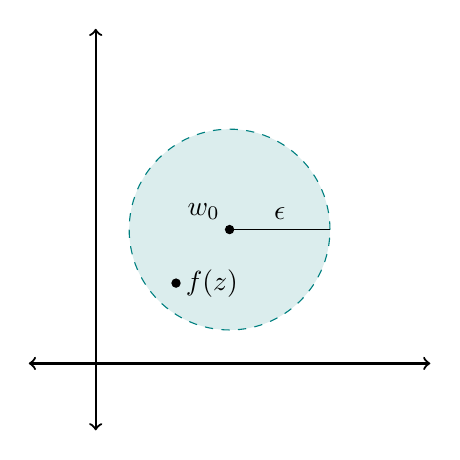
\begin{tikzpicture}[scale=0.85]
    \draw[<->,thick] (-1,0)--(5,0);
	\draw[<->,thick] (0,-1)--(0,5);
	\filldraw[teal,fill opacity=1/7,dashed](2,2) circle (1.5);
    \draw[](2,2)--(3.5,2) node[sloped,midway,above]{$\epsilon$};
    \fill (2,2) circle (2pt) node[above left]{$w_0$};
    \fill (1.2,1.2) circle (2pt) node[right]{$f(z)$};
  \end{tikzpicture}\]
In this case we write $\lim_{z \to z_0}f(z) = w_0$ or $f(z) \to w_0,\ \text{as } z \to z_0$.\\
\\
Intuitively, the limit of $f$ at $z_0$ is $w_0$ if \[\text{"$f$ is arbitrarily close to $w_0$ eventually, that is sufficiently, near $z_0$".}\] How close? Within an error of $\epsilon$. How near, eventually? Within a distance of $\delta$.
\end{definition}

\vspace*{2em}

\subsection{Problems}
\vspace{0.1in}

\begin{problem}\label{prob 4.1}\hfill
\begin{itemize}
\item[(a)] Recall that a set is open if every point of the set is an interior point. Prove that a set $U \subseteq \cc$ is open if and only if it does not contain any of its boundary points; that is, $\partial U \cap U = \emptyset$. Then deduce that the complement of a closed set is open.
\item[(b)] Prove that an open disk $D_\epsilon(z_0) = \setp{z \in \cc}{\abs{z - z_0} < \epsilon}$ is a domain; that is, a non-empty open and connected subset of $\cc$.
\end{itemize}
\end{problem}

\vspace{0.1in}

\begin{problem}\label{prob 4.2}
Sketch the sets defined by the following constraints and determine whether they are open, closed, or neither; bounded; connected. What are their boundaries?
\begin{multicols}{2}
\begin{itemize}
\item[(a)] $\abs{z + 3} < 2$.
\item[(b)] $\abs{\Im(z)} < 1$.
\item[(c)] $0 < \abs{z - 1} < 2$.
\item[(d)] $\abs{z - 1} + \abs{z + 1} = 2$.
\item[(e)] $\abs{z - 1} + \abs{z + 1} < 3$.
\item[(f)] $\abs{z} \geq \Re(z) + 1$.
\end{itemize}
\end{multicols}
\end{problem}

\vspace{0.1in}

\begin{problem}\label{prob 4.3}
Let $G$ be the set of points $z \in \cc$ satisfying either $z$ is real and $-2 < z < -1$, or $\abs{z} < 1$, or $z = 1$ or $z = 2$.
\begin{itemize}
\item[(a)] Sketch the set $G$, being careful to indicate exactly the points that are in $G$.
\item[(b)] Determine the interior points of $G$.
\item[(c)] Determine the boundary points of $G$.
\item[(d)] Determine the isolated points of $G$.
\item[(e)] $G$ can be written in three diferent ways as the union of two disjoint nonempty disconnected subsets. Describe them.
\end{itemize}
\end{problem}

\vspace*{0.1in}

\begin{problem}\label{prob 4.4}
For each of the functions below, describe the domain of definition that is understood.
\begin{multicols}{2}
\begin{itemize}
\item[(a)] $f(z) = \dfrac{1}{1 + z^2}$
\item[(b)] $f(z) = \parg\left(\dfrac{1}{z}\right)$
\item[(c)] $f(z) = \dfrac{z}{z + \overline{z}}$
\item[(d)] $f(z) = \dfrac{1}{1 - \abs{z}^2}$
\end{itemize}
\end{multicols}
\end{problem}

\vspace{0.1in}

\begin{problem}\label{prob 4.5}\hfill
\begin{itemize}
\item[(a)] Write the function $f(z) = z^3 + z + \overline{z} + 1$ in the form 
\[f(z) = u(x, y) + i\,v(x, y).\]
\item[(b)] Suppose that $f(z) = x^2 - y^2 - 2y + i(2x - 2xy)$, where $z = x + iy$. Use Proposition \ref{conjprop} (6) to write $f(z)$ in terms of $z$, and simplify the result.
\item[(c)] Write the function
\[f(z) = z + \frac{1}{z} \quad (z \neq 0)\]
in the form $f(z) = u(r,\theta) + i\,v(r,\theta)$.
\end{itemize}
\end{problem}

\vspace{0.1in}

\begin{problem}\label{prob 4.6}
Let $f : G \to \cc$ be a complex function, and suppose $z_0$ is an accumulation point of $G$. Show that 
\[\lim_{z \to z_0} f(z) = w_0 \quad \text{if and only if} \quad \lim_{z\to z_0}\abs{f(z) - w_0} = 0.\]
Thereby deduce that 
\[\lim_{z \to z_0} \bar{f}(z) = \overline{w}_0 \quad \text{if and only if} \quad \lim_{z \to z_0} f(z) = w_0.\]
\end{problem}

\vspace{0.1in}

\begin{problem}\label{prob 4.7}
Let $f : G \to \cc$ be a complex function, and suppose $z_0$ is an accumulation point of $G$. Show that 
\[\text{if }\lim_{z \to z_0} f(z) = w_0, \quad \text{then }\ \lim_{z\to z_0}\abs{f(z)} = \abs{w_0}.\]
{\footnotesize Hint. Use the reverse triangle inequality.}
\end{problem}

\vspace{0.1in}

\begin{problem}\label{prob 4.8}
Let $f : G \to \cc$ be a complex function, and suppose $z_0$ is an accumulation point of $G$. Writing $h = z - z_0$, show that 
\[\lim_{z \to z_0} f(z) = w_0 \quad \text{if and only if} \quad \lim_{h \to 0}f(z + h) = w_0.\]
\end{problem}